\anonsection{Условие лабораторной работы}
\subsection*{Задание 1}
Исследовать зависимость трудоемкости (РМ) и времени разработки (ТМ) от типа проекта (обычный, промежуточный, встроенный) для модели COCOMO. 
Получить значения PM и ТМ по всем типам проектов, приняв размер программного кода (SIZE) равным 100 KLOC.
Проанализировать как влияет на трудоемкость и время уровень способностей ключевых членов команды (драйверы ACAP – способности аналитика и PCAP – способности программиста), а также уровень автоматизации среды (драйверы MODP – использование современных методов и TOOL – использование программных инструментов). 

Результаты исследований оформить графически и сделать соответствующие выводы. 
При необходимости сократить срок выполнения проекта, что повлияет больше: способности аналитика, способности программиста или параметры среды?

\subsection*{Задание 2}
Компания получила заказ на разработку программного обеспечения для рабочей станции дизайнера автомобиля. 
Система должна иметь стандартизованный графический интерфейс, геометрические и прикладные данные должны содержаться в базе
данных (планируемый размер базы данных не более 200 тыс. записей).

При анализе проекта его размер был предварительно оценен в 140 000 строк кода. 
Проект реализуется по промежуточному варианту. 
Все показатели драйверов затрат, кроме трех имеют номинальное значение.
Знание языка программирования имеет высокую оценку, использование современных методов – очень высокую оценку и использование программных инструментов – низкую, так как используется стандартная среда визуального программирования.
Произвести оценку показателей проекта по методике СОСОМО.

\anonsection{Теоретический раздел}
Модель COCOMO (COnstructive COst MOdel) разработана Барри Боэмом. 
Это одна из основных методик, которые применяются для оценки стоимости ПО. 
Среди других методик она выгодно отличается простотой расчетов.

\textbf{Трудозатраты} рассчитываются по формуле:
\begin{equation}
	PM = C_1 * EAF * (SIZE)^{P_1}, где
\end{equation}

\begin{itemize}
	\item \textbf{PM} -- количество человеко-месяцев;
	\item \textbf{C1} -- масштабирующий коэффициент;
	\item \textbf{EAF} -- уточняющий фактор, характеризующий предметную область, персонал, среду и инструментарий, используемый для создания рабочих продуктов процесса;
	\item \textbf{SIZE} -- размер конечного продукта (кода, созданного человеком), измеряемый в исходных инструкциях (DSI), которые необходимы для реализации требуемой функциональной возможности;
	\item \textbf{P1} -- показатель степени, характеризующий экономию при больших масштабах, присущую тому процессу, который используется для создания конечного продукта;
\end{itemize}

\textbf{Время} рассчитывается по формуле:
\begin{equation}
	TM = C_2 * PM^P, где
\end{equation}

\begin{itemize}
	\item \textbf{TM} -- общее количество месяцев;
	\item \textbf{С2} -- масштабирующий коэффициент для сроков исполнения;
	\item \textbf{P} -- показатель степени, который характеризует инерцию и распараллеливание, присущее управлению разработкой ПО.
\end{itemize}

\anonsection{Задание 1}
Требуется исследовать влияние типа проекта для проекта COCOMO.

Тип проекта влияют на коэффициент, который используется для расчета параметров проекта.

В качестве атрибутов персонала использовались следующие:
\begin{enumerate}
	\item \textbf{ACAP} -- способности аналитика. Значение варьируется от 1.46 до 0.71.
	\item \textbf{PCAP} -- способности программиста. Значение варьируется от 1.42 до 0.70.
	\item \textbf{MODP} -- использование современных методов. Значение варьируется от 1.24 до 0.82.
	\item \textbf{TOOL} -- использование программных инструментов. Значение варьируется от 1.24 до 0.82.
\end{enumerate} 

Для упрощения все остальные характеристики параметра $EAF$ принимаются единице.
Размер кода для каждого из типов используется одинаковый -- 25000 строк.

Результаты в виде графиков представлены на рисунках 1-6:
\FloatBarrier
\begin{figure}[h]	
	\begin{center}
		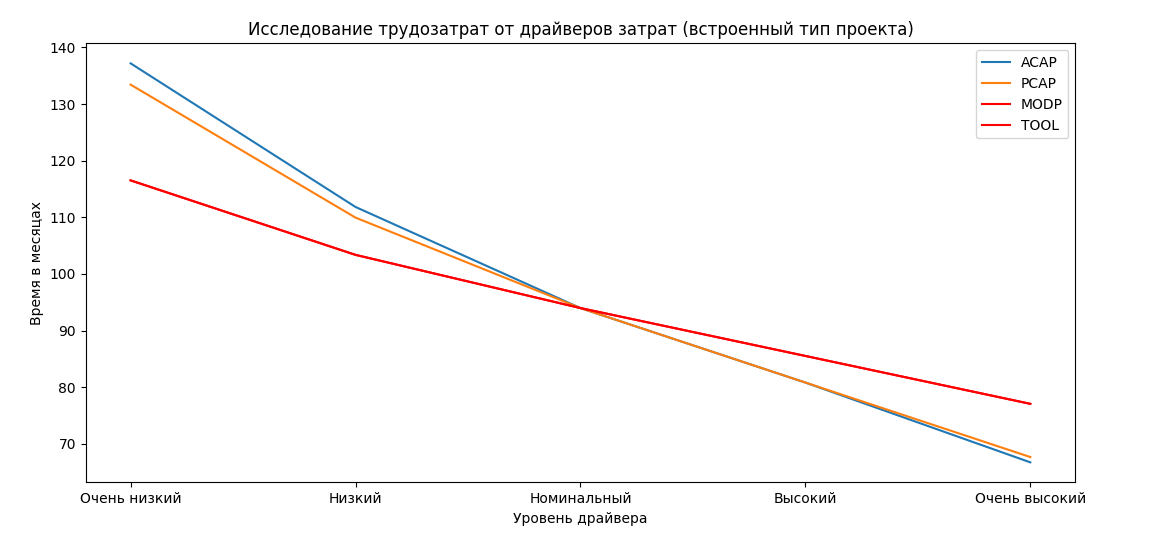
\includegraphics[width=\linewidth, height=8cm]{inc/work1.png}
	\end{center}
	\captionsetup{justification=centering}
	\caption{Исследование трудозатрат для обычного типа проекта}
\end{figure}
\FloatBarrier 

\FloatBarrier
\begin{figure}[h]	
	\begin{center}
		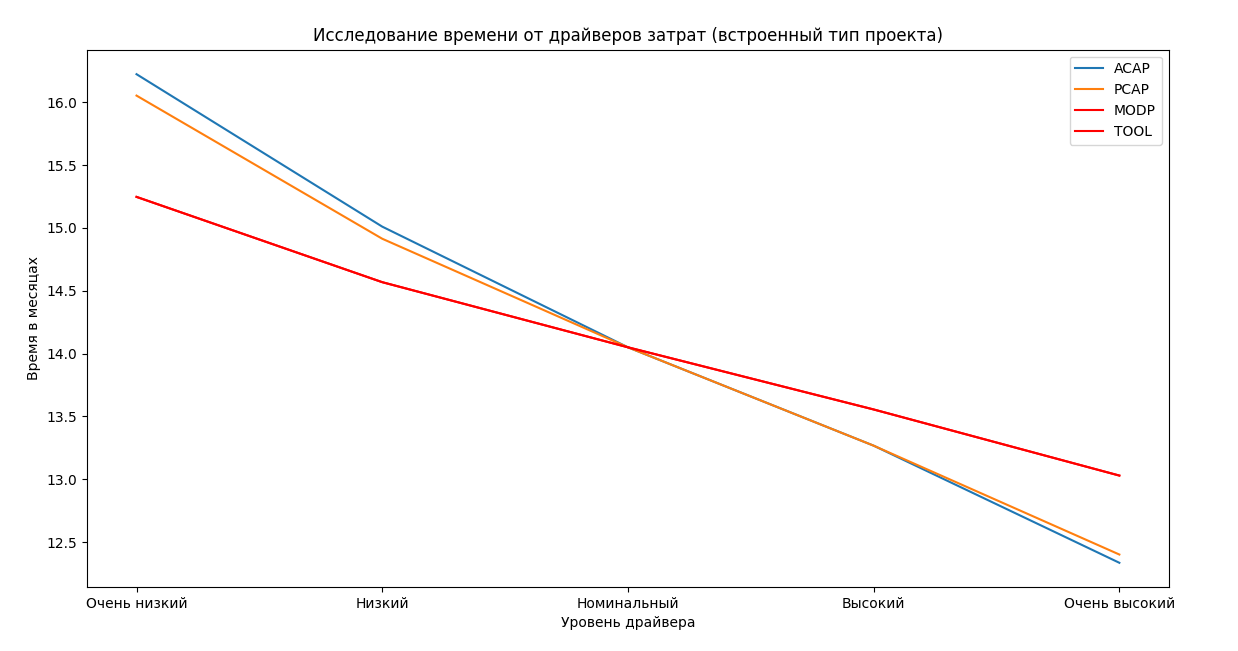
\includegraphics[width=\linewidth, height=8cm]{inc/time1.png}
	\end{center}
	\captionsetup{justification=centering}
	\caption{Исследование времени для обычного типа проекта}
\end{figure}
\FloatBarrier 

\FloatBarrier
\begin{figure}[h]	
	\begin{center}
		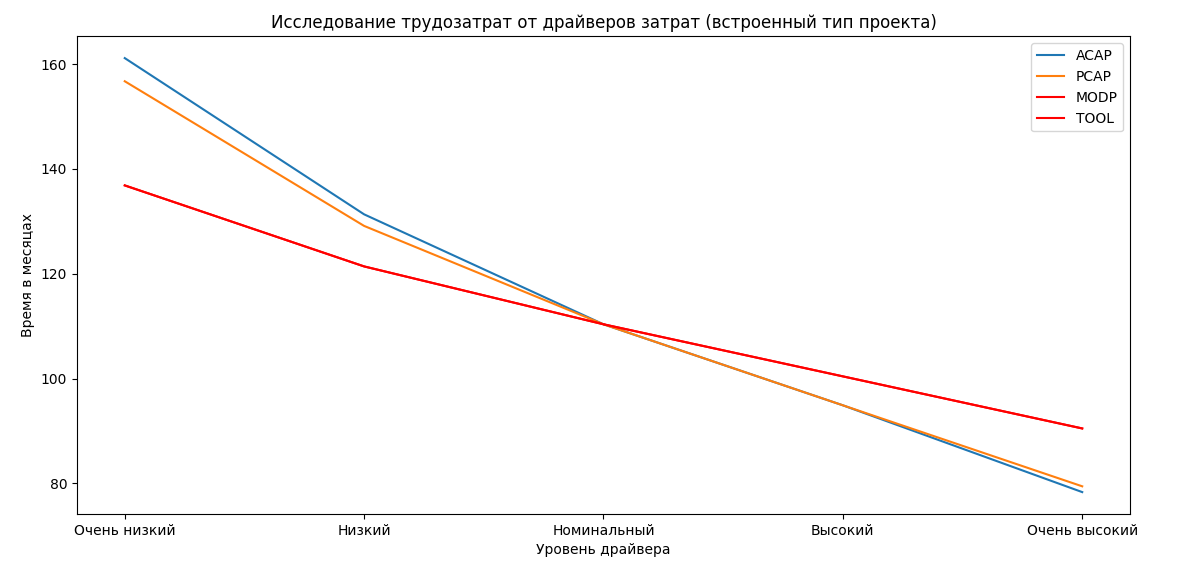
\includegraphics[width=\linewidth, height=8cm]{inc/workeasy.png}
	\end{center}
	\captionsetup{justification=centering}
	\caption{Исследование трудозатрат для промежуточного типа проекта}
\end{figure}
\FloatBarrier 

\FloatBarrier
\begin{figure}[h]	
	\begin{center}
		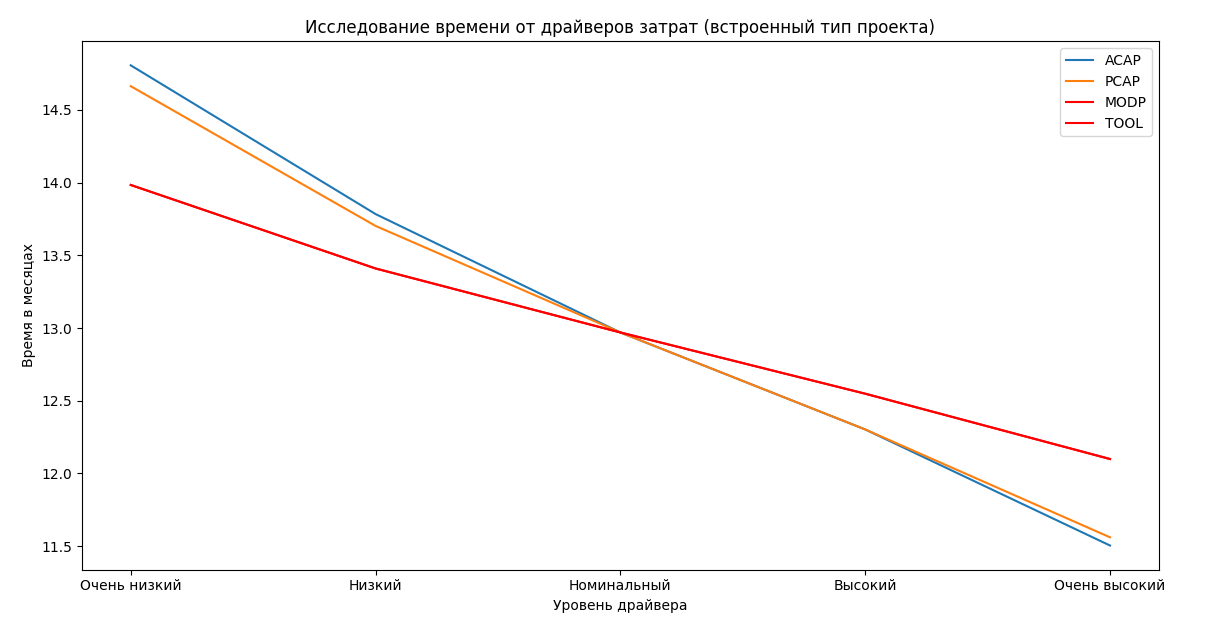
\includegraphics[width=\linewidth, height=8cm]{inc/timeeasy.png}
	\end{center}
	\captionsetup{justification=centering}
	\caption{Исследование времени для промежуточного типа проекта}
\end{figure}
\FloatBarrier 

\FloatBarrier
\begin{figure}[h]	
	\begin{center}
		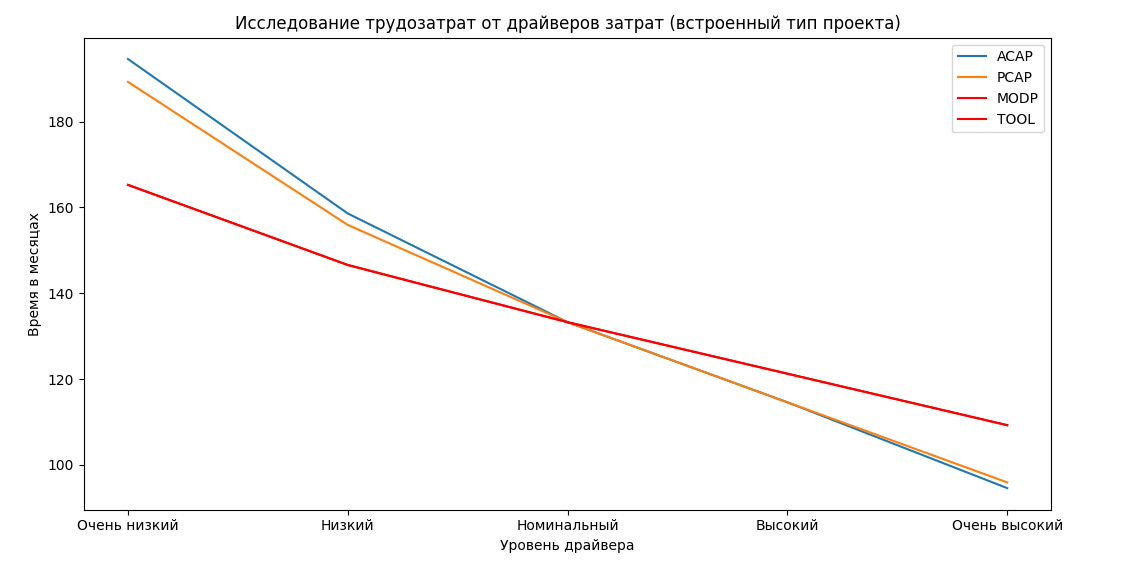
\includegraphics[width=\linewidth, height=8cm]{inc/workhard.png}
	\end{center}
	\captionsetup{justification=centering}
	\caption{Исследование трудозатрат для встроенного типа проекта}
\end{figure}
\FloatBarrier 

\FloatBarrier
\begin{figure}[h]	
	\begin{center}
		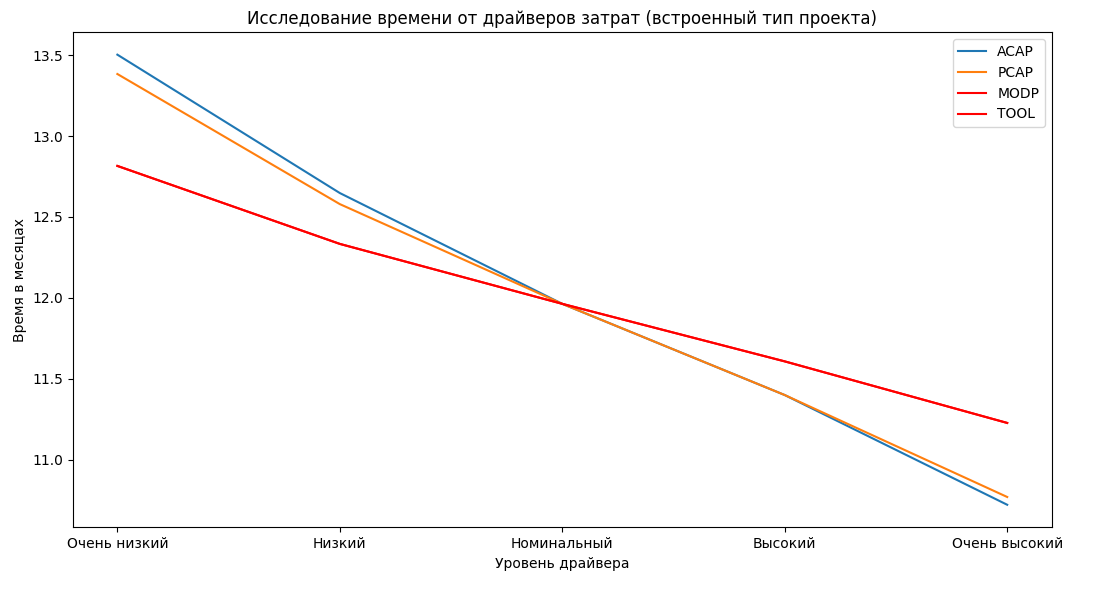
\includegraphics[width=\linewidth, height=8cm]{inc/timehard.png}
	\end{center}
	\captionsetup{justification=centering}
	\caption{Исследование времени для встроенного типа проекта}
\end{figure}
\FloatBarrier 

После анализа графиков можно сделать следующие выводы:
\begin{enumerate}
	\item Способности персонала гораздо важнее для трудозатрат и времени, чем параметры среды.
	\item Характер зависимости для проектов любой сложности одинаковый. Тем не менее, способности персонала позволяют значительно сократить время реализации проекта.
	\item Влияние способности аналитиков чуть выше, чем влияние способности программистов, но разница незначительная.
	\item В первую очередь влияют две основные характеристики: способности аналитика и способности программиста -- их и стоит улучшать для того, чтобы ускорить выполнение проекта. 
	По сравнению между очень низким и очень высоким драйверами для способностей, разница во времени достигает 25\%, в трудозатратах -- практически 50\%.
	Но так как бюджет ограничен, стоит брать людей, знакомых с приложениями -- это позволяет сократить время разработки на 25\%.
	\item Тип проекта пропорционально влияет на трудоемкость и время: трудозатраты увеличиваются на 20 человеко-месяцев при текущих параметрах проекта, время -- на 1-2 месяца.
\end{enumerate}
\anonsection{Задание 2}
Для выполнения задания был реализован графический интерфейс.
Основное меню представлено на рисунке:
\FloatBarrier
\begin{figure}[h]	
	\begin{center}
		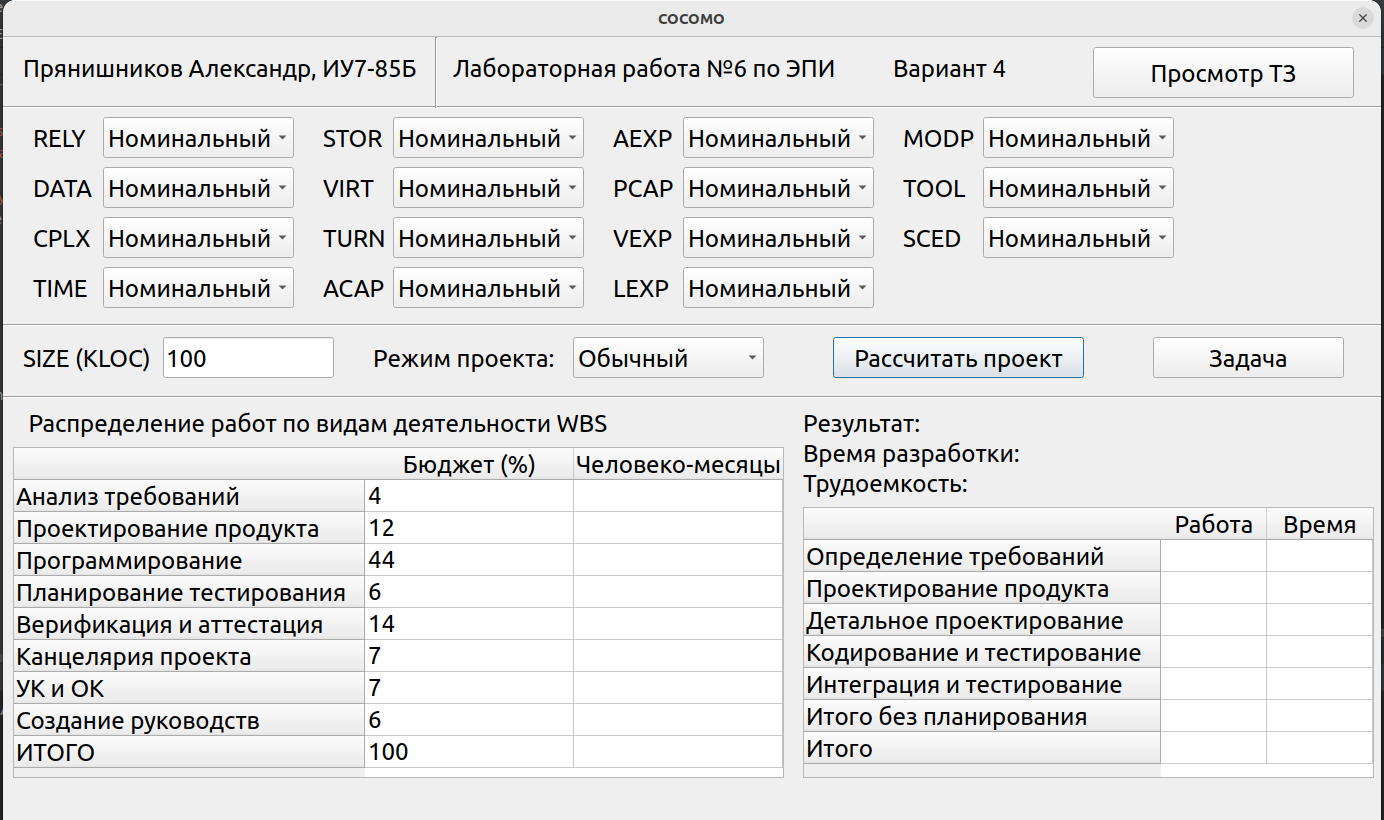
\includegraphics[width=\linewidth]{inc/prog.png}
	\end{center}
	\captionsetup{justification=centering}
	\caption{Основная программа}
\end{figure}
\FloatBarrier

В программе есть возможность рассчитывать трудоемкость и время разработки проекта для произвольных значений параметров.
По кнопке <<Задача>> можно посмотреть результаты для собственного задания.

Исходя из условия задания, коэффициенты для EAF выбраны следующим образом: $LEXP = 0.95, MODP = 0.82, TOOL = 1.1$.
Проект взят обычного типа, так как размер кода -- 140 KLOC.

\newpage
Результаты расчетов представлены на рисунке:
\FloatBarrier
\begin{figure}[h]	
	\begin{center}
		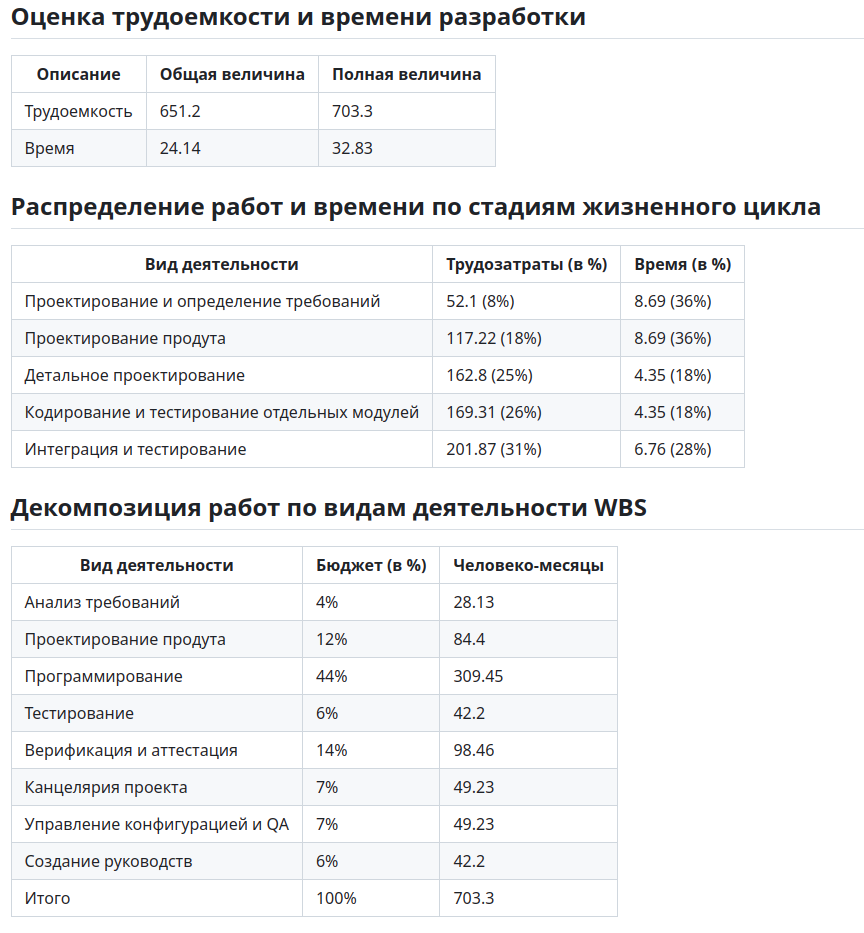
\includegraphics[width=\linewidth]{inc/table.png}
	\end{center}
	\captionsetup{justification=centering}
	\caption{Результат расчетов}
\end{figure}
\FloatBarrier 

\newpage
\anonsection{Выводы}
В результате выполнения лабораторной работы был разработан программный инструмент для оценки проекта по методике COCOMO. 
Были изучены существующие методики предварительной оценки параметров программного проекта, а также проведена практическая оценка затрат проекта.

По результатам применения методики оценки COCOMO можно заключить, что она пригодна для общей предварительной оценки всего проекта и позволяет получить приблизительные значения трудозатрат и времени на реализацию проекта, разделенные на стадии его жизненного цикла.
Однако для постоянного отслеживания состояния проекта рекомендуется использовать другие методики управления проектами с использованием различных программных средств, которые позволяют актуализировать данные проекта в реальном времени и своевременно адаптироваться к непредвиденным изменениям в проекте.